\documentclass[aspectratio=169,t]{beamer}
\usepackage[utf8]{inputenc}
\usepackage[T1]{fontenc}
\usepackage[english]{babel}
\usepackage{hyperref}
\usepackage{tikz}

\usepackage{graphicx}
\usepackage{epstopdf}
\usepackage{multirow}

\usepackage{psfrag}
\usepackage{pgfplots}
\usepackage{framed}
\usepackage{xcolor}
\usepackage{booktabs}
\usepackage{caption}
\usepackage{epstopdf}
\usepackage{amsmath}
\usepackage{tabularx}
\usepackage[]{bookmark}
%\usepackage[3D]{movie15}
%\usepackage{media9}
\usepackage[binary-units,abbreviations]{siunitx}
\usepackage[textfont=normalsize, labelfont=normalsize, justification=centering]{subcaption}
\usepackage{marvosym}
\usepackage{calc}
\usepackage{color, colortbl}
\usepackage[]{svg} 
\usepackage[]{trfsigns} 
\usepackage[nomessages]{fp}
\usepackage[]{csquotes}\MakeOuterQuote{"}
\selectcolormodel{rgb}

\makeatletter
\def\beamer@calltheme#1#2#3{\def\beamer@themelist{#2}
	\@for\beamer@themename:=\beamer@themelist\do
	{\usepackage[{#1}]{\beamer@themelocation/#3\beamer@themename}}}
\def\usefolder#1{\def\beamer@themelocation{#1}}
\def\beamer@themelocation{}
\usefolder{theme}

\usetikzlibrary{matrix,
	decorations.pathreplacing,
	calc,
	positioning,
	external,
	3d,
	shapes,
	arrows,
	pgfplots.statistics}
\pgfplotsset{compat=1.16}
\tikzstyle{faunode}=[rounded corners, draw=faublue, fill=faublue!10,  align=center, inner sep=0.3cm, line width=0.4mm]
\tikzstyle{fauellipseFixedWidth}=[ellipse, draw=faublue, fill=faublue!10,  align=center, inner sep=0.3cm, line width=0.4mm, minimum width=3cm]
\tikzstyle{fauellipse}=[ellipse, draw=faublue, fill=faublue!10,  align=center, inner sep=0.3cm, line width=0.4mm]
\tikzstyle{fauarrow}=[draw=faublue,->, line width=0.4mm]
\tikzstyle{fauline}=[draw=faublue, line width=0.4mm]


\usepackage[backend=bibtex,sorting=none,doi=true,style=phys]{biblatex}
%\usepackage[]{biblatex}
\bibliography{./references}

% Themes:
%  - fau:          FAU theme
%  - fau-tf:       TechFak FAU theme
%  - fau-tf-lme:   TechFak LME FAU theme
%
% Options:
%  - image:        Cover image on title page
%  - plain:        Plain title page
%  - longtitle:    Title page layout for long title
\usetheme[longtitle]{fau-tf-lme}

% END of THEME SETTINGS
% --------------------------------------------------------------------------------------------------------------------------------------------------------------------------

\sisetup{
exponent-product =\ensuremath{{\,\cdot\,}}
}

% Enable semi-transparent animation preview
\setbeamercovered{transparent}
\setbeamertemplate{blocks}[rounded]
\captionsetup{labelformat=empty,labelsep=none, labelfont=normalsize, justification=centering}


\newcommand\Wider[2][1.0cm]{%
\makebox[\linewidth][c]{%
  \begin{minipage}{\dimexpr\textwidth+#1\relax}
  \raggedright#2
  \end{minipage}%
  }%
}


\let\origitem\item
\renewcommand{\item}{\normalfont\origitem}
\newcommand{\bluefat}[1]{\textcolor{faublue}{\textbf{#1}}}
\newcommand{\bolditem}{\normalfont\origitem\bfseries}
\newcommand{\question}{{\bf Question: }}
\newcommand{\answer}{{\bf Answer: }}
\newcommand{\myExample}{{\bf Example }}
\newcommand{\real}{\mbox{${\mathbb R}$}}
\definecolor{defColor}{rgb}{0.8,0.87,0.97}
\definecolor{defColorT}{rgb}{0,0,0}
\definecolor{defColorF}{rgb}{1,1,1}
\newenvironment{myDefinition}{%
	\def\FrameCommand{\fboxsep=\FrameSep{} \fcolorbox{defColorF}{defColor}}%
	\color{defColorT}\MakeFramed{\FrameRestore{}}}%
{\endMakeFramed}

% Title page
\title[Medical Engineering II]{Medical Engineering - Imaging Systems}
\author{Prof.\ Dr.-Ing.\ habil.\ Andreas Maier}
\date{SS 2021}
\institute{Pattern Recognition Lab (CS 5)}

\newcommand{\password}{\texttt{mt2\_ss21}}


\AtBeginSection[]{
	{
		\setbeamertemplate{footline}{}
		\begin{frame}[noframenumbering]{\insertsubtitle}
			 \tableofcontents[currentsection]
		\end{frame} 
	}
}
\AtBeginSubsection[]{
	{

		\setbeamertemplate{footline}{}
		\begin{frame}[noframenumbering]{\insertsubtitle}
			 \tableofcontents[currentsection, currentsubsection]
		\end{frame} 
	}
}


\usepackage[]{subcaption} 

\renewcommand{\vec}[1]{\boldsymbol{#1}}
\newcommand{\mat}[1]{\boldsymbol{#1}}

\newcommand\B[1]{\ensuremath{\vec{B}_{#1}}}

\def\longtime{\ensuremath{T_1}}						% T1
\def\transtime{\ensuremath{T_2}}						% T2
\def\inhomogtime{\ensuremath{\transtime^*}}						% T2*

\def\spatialfreq{\ensuremath{s}}      % Spatial frequency

\def\larmorfreq{\ensuremath{f_\ell}}  % Larmor frequency

\def\hydrogen{\ensuremath{{}^1\textrm{H}}} % Hydrogen

\def\magn{\ensuremath{\vec M}}
\def\magnzero{\ensuremath{\magn_0}}
\def\magnlong{\ensuremath{\magn_z}} % Longitudinal magnetization
\def\magntrans{\ensuremath{\magn_{xy}}} % Transversal magnetization


\subtitle{Magnetic Resonance II}
\author{Prof.\ Andreas Maier, Jens Wetzl, Felix Lugauer}


\begin{document}

\frame[plain]{\titlepage}

\begin{frame}
  \frametitle{Magnetic Resonance 2}
  
  \tableofcontents
\end{frame}

\section{Principles of Magnetic Resonance Imaging}% (fold)
\label{sec:principles_of_magnetic_resonance_imaging}

\begin{frame}
	\frametitle{Magnetic Resonance {\color{red}Imaging}}
	
	\begin{itemize}
		\item So far: excitation of and signal reception from all \hydrogen{} nuclei \\ within the magnetic field
		\item For \emph{imaging}, we need spatial information
		\item Two concepts:
		\begin{itemize}
			\item \emph{Slice Selection} to restrict excitation to a slice
			\item \emph{Spatial Encoding} to encode spatial information \\ within a slice or volume
		\end{itemize}
		\item Both are based on the gradient coil system
	\end{itemize}
\end{frame}

\begin{frame}
	\frametitle{Components of an MRI Scanner}
	
	\begin{center}
		\includegraphics[height=0.8\textheight]{images/mri_scanner}
	\end{center}
	
	{\flushright
	\tiny Image source: \url{http://www.magnet.fsu.edu}}
\end{frame}

\begin{frame}
	\frametitle{Gradient Coil System}
	
	\begin{itemize}
		\item Main magnetic field \B0 is (theoretically) homogeneous
		\item Gradient coils allow linear variation of the magnetic field
		\item Installed in 3 orthogonal directions, combination allows \\ linear variation in arbitrary directions
		\item $\rightarrow$ Arbitrary slice orientations, as opposed to CT
	\end{itemize}
	
	\begin{center}
		\includegraphics[height=0.4\textheight]{images/gradients}
		
		{\scriptsize Image source: Slides ``Bildgebende Verfahren in der Medizin'', Springer Berlin Heidelberg}
	\end{center}
	
\end{frame}

\begin{frame}
	\frametitle{Gradient Coil System}
	
	\begin{center}
		\includegraphics[height=0.8\textheight]{images/mri_scannercoils}
	\end{center}
	
	{\scriptsize Image source: \url{http://www.magnet.fsu.edu}}
\end{frame}




\subsection{Slice Selection} % (fold)
\label{sub:slice_selection}

\begin{frame}
	\frametitle{Slice Selection I}
	
	\begin{itemize}
		\item Linear variation of \B0 in head-feet direction ($z$)
		\item $\rightarrow$ Larmor frequency \larmorfreq{} dependent on offset in $z$ direction:
		$$\larmorfreq(z) = \gamma \cdot \left( \Vert \B0 \Vert + z \right)$$
	\end{itemize}
	
	\begin{center}
		\begingroup
		\tikzset{every picture/.style={scale=0.5}}%
		\tikzsetnextfilename{mr_slice_selection_field}
\begin{tikzpicture}
	\draw[->] (0, 0) -- (5, 0) node [right] {$z$};
	\draw[->] (0, 0) -- (0, 4) node [above] {$\larmorfreq(z)$};
	\draw (0.5,0.5) -- (4,4);
	\draw (1, -1) circle (1.5ex) node [left=2ex, anchor=east] {head};
	%\draw (1.5, -1) -- (2, -1.25); % arms
	%\draw (1.5, -1) -- (2, -0.85); % arms
	\draw (1, -1) ++(1.5ex, 0) -- (4, -1) node [right=1ex] {feet} -- (4,-0.5) -- (3.75, -1);
	%\draw[fill=white] (2.1, -0.75) node (A1) {} -- (2.5, -0.25) node (B1) {} -- (2.5, -1.25) node (C1) {} -- (2.1, -1.75) node (D1) {} -- cycle;
	%\draw[fill=white] (2.5, -0.75) node (A2) {} -- (2.9, -0.25) node (B2) {} -- (2.9, -1.25) node (C2) {} -- (2.5, -1.75) node (D2) {} -- cycle;
	%\draw[fill=white] (A1.center) -- (A2.center) -- (B2.center) -- (B1.center) -- cycle;
	%\draw[fill=white] (A1.center) -- (A2.center) -- (D2.center) -- (D1.center) -- cycle;
	%\draw (2.7, -1) -- (2.9, -1);
	%\draw[densely dashed] (2.3, -0.5) -- (2.3,2.3) -- ++(-2.3,0);
	%\draw[densely dashed] (2.7, -0.5) -- (2.7,2.7) -- ++(-2.7,0);
	%\draw[fill=black] (2.3, 0) circle (1.5pt) node [above left] {$z_1$};
	%\draw[fill=black] (2.7, 0) circle (1.5pt) node [above right] {$z_2$};
	%\draw[fill=black] (0, 2.3) circle (1.5pt) node [left] {$\larmorfreq(z_1)$};
	%\draw[fill=black] (0, 2.7) circle (1.5pt) node [left] {$\larmorfreq(z_2)$};
	%\draw[<->, shorten >=1pt, shorten <=1pt] ($(A1.center)!0.5!(D1.center)$) -- node (mid) {} ($(A2.center)!0.5!(D2.center)$);
	%\draw[shorten <=2pt] (mid.center) to[out=270] ++(0.75, -0.2) node [right] {slice thickness};
\end{tikzpicture}
		\endgroup
	\end{center}
	
	\begin{itemize}
		\item $z$ direction is an example, works in arbitrary oblique orientations!
	\end{itemize}
\end{frame}

\begin{frame}
	\frametitle{Slice Selection II}
	
	\begin{itemize}
		\item Excitation of a slice from position $z_1$ to $z_2$: use RF waves with frequencies in the range of $\larmorfreq(z_1)$ to $\larmorfreq(z_2)$
	\end{itemize}
	
	\begin{center}
		\begingroup
		\tikzset{every picture/.style={scale=0.8}}
		\input{tikz/slice_selection.tikz}
		\endgroup
	\end{center}
\end{frame}

% subsection slice_selection (end)



\subsection{Spatial Encoding} % (fold)
\label{sub:spatial_encoding}

\begin{frame}
	\frametitle{Spatial Encoding}
	
	\begin{itemize}
		\item Unfortunately, the slice selection principle cannot be extended to encode spatial locations within a slice
		\item Even with multiple gradient fields, selection is always a plane (possibly oblique), not a single point
		
		\vspace{2ex}
		
		\item Recall: magnetization vectors precess in the transversal plane
		\item Make use of the \textbf{phase shift} between them to encode location
		
		\begin{center}
			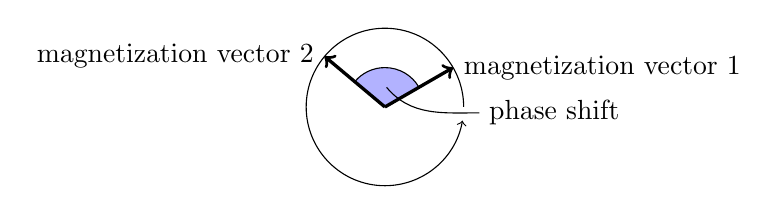
\begin{tikzpicture}
				\fill[blue!30!white] (0, 0) -- (30:0.5) arc (30:140:0.5) -- cycle;
				\draw[->] (1, 0) arc (0:350:1);
				\draw[very thick,->] (0, 0) -- (30:1) node [right] {magnetization vector 1};
				\draw[very thick,->] (0, 0) -- (140:1) node [left] {magnetization vector 2};
				\draw (30:0.5) arc (30:140:0.5);
				\draw (85:0.25) to[out=310,in=180] (1.2, -0.075) node [right] {phase shift};
			\end{tikzpicture}
		\end{center}
	\end{itemize}
\end{frame}

\begin{frame}
	\frametitle{One-Dimensional Example}
	
	\begin{itemize}
		\item Exemplary explanation for encoding 1-D locations first
		\item Extension to $n$-D later on
		\item 1-D example ``image'' with more hydrogen nuclei towards the boundaries, represented by the magnitudes of the vectors:
	\end{itemize}
	
	\begin{center}
		\begingroup
		\tikzset{every picture/.style={scale=0.9}}
		\tikzsetnextfilename{mr_spatial_encoding_voxels}
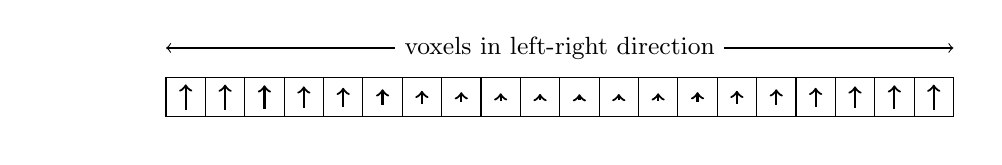
\begin{tikzpicture}[scale=0.5]
	\draw[white] (-4, -1) rectangle (20, 1);
	\pgfmathsetmacro{\angle}{0}
	\foreach \idx in {0,1,...,19} {
		\draw ($(\idx,0)-(0.5,0.5)$) rectangle ($(\idx,0)+(0.5,0.5)$);
		\pgfmathsetmacro{\anglevalue}{90+\idx*\angle}
		\pgfmathsetmacro{\magn}{0.125*(cos(\idx*360/20) + 1)+0.075}
		\pgfmathsetmacro{\x}{\idx+\magn*cos(\anglevalue)}
		\pgfmathsetmacro{\a}{\idx-\magn*cos(\anglevalue)}
		\pgfmathsetmacro{\y}{\magn*sin(\anglevalue)}
		\pgfmathsetmacro{\b}{-\magn*sin(\anglevalue)}
		\draw[thick,<-] (\x, \y) -- (\a, \b);
	}
	\draw[<->] (-0.5, 1.25) -- node [fill=white,font=\small] {voxels in left-right direction} (19.5, 1.25);
\end{tikzpicture}
		\endgroup
	\end{center}
	
	\begin{itemize}
		\item Directly after excitation, all spins have the same phase
	\end{itemize}
\end{frame}

\begin{frame}
	\frametitle{Net Magnetization}
	
	\begin{itemize}
		\item Measurable quantity in MR scanners: net magnetization
	\end{itemize}
	
	\begin{center}
		\begingroup
		\tikzset{every picture/.style={scale=0.9}}
		\tikzsetnextfilename{mr_spatial_encoding_net_magnetization}
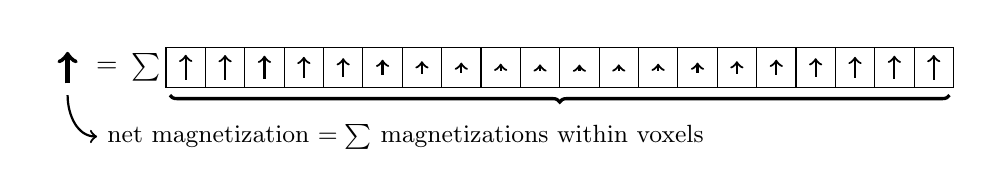
\begin{tikzpicture}[scale=0.5]
	\draw[white] (-4, -1) rectangle (20, 1);
	\draw (-1, 0) node {$\sum$};
	\draw (-2, 0) node {$=$};
	\draw[ultra thick,->] (-3, -0.4) -- (-3,0.4);
	\pgfmathsetmacro{\angle}{0}
	\foreach \idx in {0,1,...,19} {
		\draw ($(\idx,0)-(0.5,0.5)$) rectangle ($(\idx,0)+(0.5,0.5)$);
		\pgfmathsetmacro{\anglevalue}{90+\idx*\angle}
		\pgfmathsetmacro{\magn}{0.125*(cos(\idx*360/20) + 1)+0.075}
		\pgfmathsetmacro{\x}{\idx+\magn*cos(\anglevalue)}
		\pgfmathsetmacro{\a}{\idx-\magn*cos(\anglevalue)}
		\pgfmathsetmacro{\y}{\magn*sin(\anglevalue)}
		\pgfmathsetmacro{\b}{-\magn*sin(\anglevalue)}
		\draw[thick,<-] (\x, \y) -- (\a, \b);
	}
	\draw[very thick,decoration={brace, mirror},decorate] (-0.4, -0.7) -- (19.4, -0.7);
	\draw[->,thick] (-3, -0.7) to[out=270,in=180] (-2.25, -1.75) node [right,font=\small] {net magnetization $= \sum$ magnetizations within voxels};
\end{tikzpicture}
		\endgroup
	\end{center}
	
\end{frame}

\begin{frame}
	\frametitle{Precession}
	
	\begin{itemize}
		\item Ignore relaxation for now
		\item Assume a homogeneous magnetic field without gradients
		\item[$\rightarrow$] Spins precess at the same Larmor frequency and net magnetziation is unchanged
	\end{itemize}
	
	\begin{center}
		\begingroup
		\tikzset{every picture/.style={scale=0.9}}
		\tikzsetnextfilename{mr_spatial_encoding_precession}
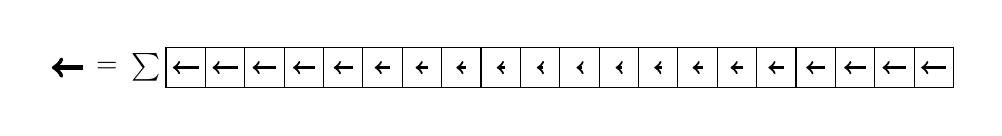
\begin{tikzpicture}[scale=0.5]
	\draw[white] (-4, -1) rectangle (20, 1);
	\draw (-1, 0) node {$\sum$};
	\draw (-2, 0) node {$=$};
	\draw[ultra thick,->] (-2.6, 0) -- (-3.4,0);
	\pgfmathsetmacro{\angle}{0}
	\pgfmathsetmacro{\startangle}{180}
	\foreach \idx in {0,1,...,19} {
		\draw ($(\idx,0)-(0.5,0.5)$) rectangle ($(\idx,0)+(0.5,0.5)$);
		\pgfmathsetmacro{\anglevalue}{\startangle+\idx*\angle}
		\pgfmathsetmacro{\magn}{0.125*(cos(\idx*360/20) + 1)+0.075}
		\pgfmathsetmacro{\x}{\idx+\magn*cos(\anglevalue)}
		\pgfmathsetmacro{\a}{\idx-\magn*cos(\anglevalue)}
		\pgfmathsetmacro{\y}{\magn*sin(\anglevalue)}
		\pgfmathsetmacro{\b}{-\magn*sin(\anglevalue)}
		\draw[thick,<-] (\x, \y) -- (\a, \b);
	}
\end{tikzpicture}
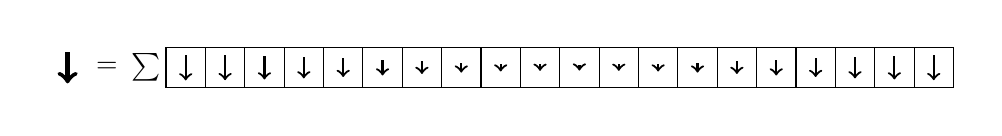
\begin{tikzpicture}[scale=0.5]
	\draw[white] (-4, -1) rectangle (20, 1);
	\draw (-1, 0) node {$\sum$};
	\draw (-2, 0) node {$=$};
	\draw[ultra thick,<-] (-3, -0.4) -- (-3,0.4);
	\pgfmathsetmacro{\angle}{0}
	\pgfmathsetmacro{\startangle}{270}
	\foreach \idx in {0,1,...,19} {
		\draw ($(\idx,0)-(0.5,0.5)$) rectangle ($(\idx,0)+(0.5,0.5)$);
		\pgfmathsetmacro{\anglevalue}{\startangle+\idx*\angle}
		\pgfmathsetmacro{\magn}{0.125*(cos(\idx*360/20) + 1)+0.075}
		\pgfmathsetmacro{\x}{\idx+\magn*cos(\anglevalue)}
		\pgfmathsetmacro{\a}{\idx-\magn*cos(\anglevalue)}
		\pgfmathsetmacro{\y}{\magn*sin(\anglevalue)}
		\pgfmathsetmacro{\b}{-\magn*sin(\anglevalue)}
		\draw[thick,<-] (\x, \y) -- (\a, \b);
	}
\end{tikzpicture}
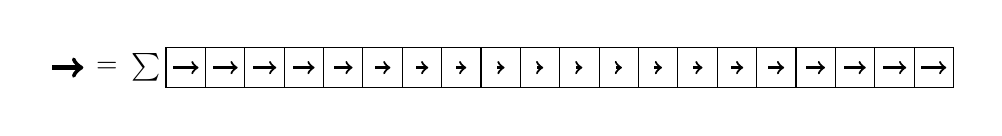
\begin{tikzpicture}[scale=0.5]
	\draw[white] (-4, -1) rectangle (20, 1);
	\draw (-1, 0) node {$\sum$};
	\draw (-2, 0) node {$=$};
	\draw[ultra thick,<-] (-2.6, 0) -- (-3.4,0);
	\pgfmathsetmacro{\angle}{0}
	\pgfmathsetmacro{\startangle}{0}
	\foreach \idx in {0,1,...,19} {
		\draw ($(\idx,0)-(0.5,0.5)$) rectangle ($(\idx,0)+(0.5,0.5)$);
		\pgfmathsetmacro{\anglevalue}{\startangle+\idx*\angle}
		\pgfmathsetmacro{\magn}{0.125*(cos(\idx*360/20) + 1)+0.075}
		\pgfmathsetmacro{\x}{\idx+\magn*cos(\anglevalue)}
		\pgfmathsetmacro{\a}{\idx-\magn*cos(\anglevalue)}
		\pgfmathsetmacro{\y}{\magn*sin(\anglevalue)}
		\pgfmathsetmacro{\b}{-\magn*sin(\anglevalue)}
		\draw[thick,<-] (\x, \y) -- (\a, \b);
	}
\end{tikzpicture} \\
		$\vdots$
		\endgroup
	\end{center}
\end{frame}

\begin{frame}
	\frametitle{Applying a Gradient Field}
	
	\begin{columns}[onlytextwidth,c]
		\column{.3\linewidth}
		\column{.7\linewidth}
		\begin{itemize}
			\item With a gradient field, magnetization vectors precess at different speeds
			\item They accumulate a phase shift
			\item Measurable net magnetization changes
		\end{itemize}
	\end{columns}
	
	
	
	\begin{center}
		\begingroup
		\tikzset{every picture/.style={scale=0.9}}
		\input{tikz/spatial_encoding_gradient.tikz}
		\endgroup
	\end{center}
	
\end{frame}

\begin{frame}
	\frametitle{Phase ``Patterns''}
	
	\begin{itemize}
		\item May seem counterproductive, but is core idea of spatial encoding!
		
		\vspace{1ex}
		
		\item  If hydrogen nuclei distribution matches ``pattern'' implied by the phase shift $\rightarrow$ measurable net magnetization
	\end{itemize}
	
	\vspace{-2ex}
	
	\begin{center}
		\begingroup
		\tikzset{every picture/.style={scale=0.9}}
		\tikzsetnextfilename{mr_spatial_encoding_pattern_1}
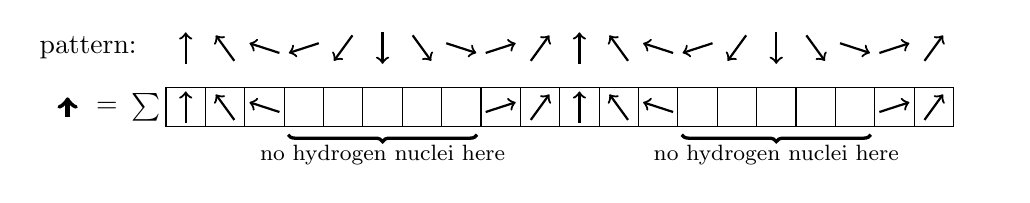
\begin{tikzpicture}[scale=0.5]
	\draw[white] (-4, -1) rectangle (20, 1);
	\draw (-1, 0) node {$\sum$};
	\draw (-2, 0) node {$=$};
	\draw (-1, 1.5) node [anchor=east] {pattern:};
	\draw[ultra thick,->] (-3, -0.25) -- (-3,0.25);
	\pgfmathsetmacro{\angle}{36}
	\pgfmathsetmacro{\startangle}{90}
	\foreach \idx in {0,1,...,19} {
		\pgfmathsetmacro{\anglevalue}{\startangle+\idx*\angle}
		\pgfmathsetmacro{\x}{\idx+0.4*cos(\anglevalue)}
		\pgfmathsetmacro{\a}{\idx-0.4*cos(\anglevalue)}
		\pgfmathsetmacro{\y}{1.5+0.4*sin(\anglevalue)}
		\pgfmathsetmacro{\b}{1.5+-0.4*sin(\anglevalue)}
		\draw[thick,<-] (\x, \y) -- (\a, \b);
	}
	\foreach \idx in {0,1,...,19} {
		\draw ($(\idx,0)-(0.5,0.5)$) rectangle ($(\idx,0)+(0.5,0.5)$);
	}
	\foreach \idx in {0,1,2,8,9,10,11,12,18,19} {
		\pgfmathsetmacro{\anglevalue}{\startangle+\idx*\angle}
		\pgfmathsetmacro{\x}{\idx+0.4*cos(\anglevalue)}
		\pgfmathsetmacro{\a}{\idx-0.4*cos(\anglevalue)}
		\pgfmathsetmacro{\y}{0.4*sin(\anglevalue)}
		\pgfmathsetmacro{\b}{-0.4*sin(\anglevalue)}
		\draw[thick,<-] (\x, \y) -- (\a, \b);
	}
	\draw[very thick,decoration={brace, mirror},decorate] (2.6, -0.7) -- node [below,font=\small] {\parbox{5.5cm}{\centering {\footnotesize no hydrogen nuclei here}}} (7.4, -0.7);
	\draw[very thick,decoration={brace, mirror},decorate] (12.6, -0.7) -- node [below,font=\small] {\parbox{5.5cm}{\centering {\footnotesize no hydrogen nuclei here}}} (17.4, -0.7);
\end{tikzpicture}
		\endgroup
	\end{center}
	\uncover<2>{
	\begin{itemize}
		\item Better match $\rightarrow$ higher net magnetization
	\end{itemize}
	\begin{center}
		\begingroup
		\tikzset{every picture/.style={scale=0.9}}
		\tikzsetnextfilename{mr_spatial_encoding_pattern_2}
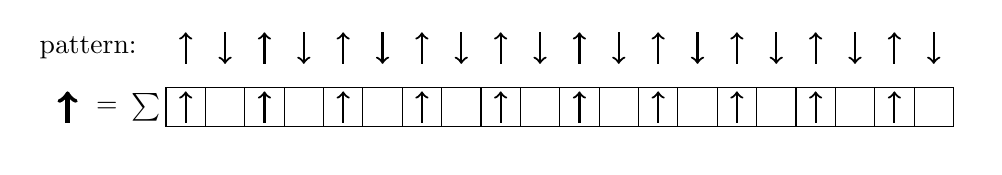
\begin{tikzpicture}[scale=0.5]
	\draw[white] (-4, -1) rectangle (20, 1);
	\draw (-1, 0) node {$\sum$};
	\draw (-2, 0) node {$=$};
	\draw (-1, 1.5) node [anchor=east] {pattern:};
	\draw[ultra thick,->] (-3, -0.4) -- (-3,0.4);
	\pgfmathsetmacro{\angle}{180}
	\pgfmathsetmacro{\startangle}{90}
	\foreach \idx in {0,1,...,19} {
		\pgfmathsetmacro{\anglevalue}{\startangle+\idx*\angle}
		\pgfmathsetmacro{\x}{\idx+0.4*cos(\anglevalue)}
		\pgfmathsetmacro{\a}{\idx-0.4*cos(\anglevalue)}
		\pgfmathsetmacro{\y}{1.5+0.4*sin(\anglevalue)}
		\pgfmathsetmacro{\b}{1.5+-0.4*sin(\anglevalue)}
		\draw[thick,<-] (\x, \y) -- (\a, \b);
	}
	\foreach \idx in {0,1,...,19} {
		\draw ($(\idx,0)-(0.5,0.5)$) rectangle ($(\idx,0)+(0.5,0.5)$);
	}
	\foreach \idx in {0,2,...,18} {
		\pgfmathsetmacro{\anglevalue}{\startangle+\idx*\angle}
		\pgfmathsetmacro{\x}{\idx+0.4*cos(\anglevalue)}
		\pgfmathsetmacro{\a}{\idx-0.4*cos(\anglevalue)}
		\pgfmathsetmacro{\y}{0.4*sin(\anglevalue)}
		\pgfmathsetmacro{\b}{-0.4*sin(\anglevalue)}
		\draw[thick,<-] (\x, \y) -- (\a, \b);
	}
\end{tikzpicture}
		\endgroup
	\end{center}}
\end{frame}

\begin{frame}
	\frametitle{Spatial Encoding}
	
	\begin{columns}[onlytextwidth,c]
		\column{.45\linewidth}
		{\small
		\begin{itemize}
			\item Apply different gradients
			\item Measure net magnetization
		\end{itemize}}
		\column{.55\linewidth}
		{\small
		\begin{itemize}
			\item[$\rightarrow$] creates different phase patterns
			\item[$\rightarrow$] describes similarity to each pattern
		\end{itemize}}
	\end{columns}
	\begin{center}
		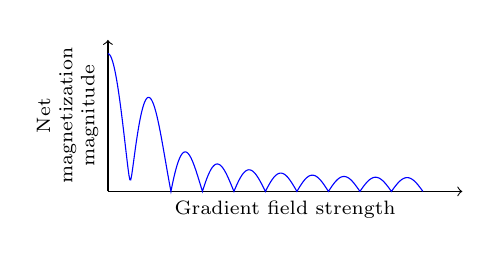
\begin{tikzpicture}[yscale=3.5]
   		\draw[->] (0, 0) -- node [below, font=\scriptsize] {\parbox{3cm}{\centering Gradient field strength}} (4.5, 0);
   		\draw[->] (0, 0) -- node [above, sloped, font=\scriptsize] {\parbox{2cm}{\centering Net magnetization \\ magnitude}} (0, 0.55);
   		\draw[blue] (0.000000, 0.500000)
    -- (0.011111, 0.498993)
    -- (0.022222, 0.495976)
    -- (0.033333, 0.490965)
    -- (0.044444, 0.483986)
    -- (0.055556, 0.475075)
    -- (0.066667, 0.464278)
    -- (0.077778, 0.451650)
    -- (0.088889, 0.437256)
    -- (0.100000, 0.421170)
    -- (0.111111, 0.403476)
    -- (0.122222, 0.384266)
    -- (0.133333, 0.363639)
    -- (0.144444, 0.341703)
    -- (0.155556, 0.318575)
    -- (0.166667, 0.294377)
    -- (0.177778, 0.269242)
    -- (0.188889, 0.243312)
    -- (0.200000, 0.216740)
    -- (0.211111, 0.189698)
    -- (0.222222, 0.162386)
    -- (0.233333, 0.135060)
    -- (0.244444, 0.108093)
    -- (0.255556, 0.082163)
    -- (0.266667, 0.058836)
    -- (0.277778, 0.042508)
    -- (0.288889, 0.041785)
    -- (0.300000, 0.056652)
    -- (0.311111, 0.078109)
    -- (0.322222, 0.101488)
    -- (0.333333, 0.125154)
    -- (0.344444, 0.148430)
    -- (0.355556, 0.170963)
    -- (0.366667, 0.192530)
    -- (0.377778, 0.212971)
    -- (0.388889, 0.232162)
    -- (0.400000, 0.250000)
    -- (0.411111, 0.266400)
    -- (0.422222, 0.281290)
    -- (0.433333, 0.294611)
    -- (0.444444, 0.306315)
    -- (0.455556, 0.316366)
    -- (0.466667, 0.324735)
    -- (0.477778, 0.331407)
    -- (0.488889, 0.336374)
    -- (0.500000, 0.339639)
    -- (0.511111, 0.341215)
    -- (0.522222, 0.341122)
    -- (0.533333, 0.339392)
    -- (0.544444, 0.336064)
    -- (0.555556, 0.331184)
    -- (0.566667, 0.324809)
    -- (0.577778, 0.317001)
    -- (0.588889, 0.307829)
    -- (0.600000, 0.297371)
    -- (0.611111, 0.285709)
    -- (0.622222, 0.272931)
    -- (0.633333, 0.259128)
    -- (0.644444, 0.244400)
    -- (0.655556, 0.228845)
    -- (0.666667, 0.212568)
    -- (0.677778, 0.195676)
    -- (0.688889, 0.178275)
    -- (0.700000, 0.160475)
    -- (0.711111, 0.142386)
    -- (0.722222, 0.124116)
    -- (0.733333, 0.105773)
    -- (0.744444, 0.087465)
    -- (0.755556, 0.069296)
    -- (0.766667, 0.051369)
    -- (0.777778, 0.033781)
    -- (0.788889, 0.016628)
    -- (0.800000, 0.000000)
    -- (0.811111, 0.016017)
    -- (0.822222, 0.031342)
    -- (0.833333, 0.045901)
    -- (0.844444, 0.059624)
    -- (0.855556, 0.072450)
    -- (0.866667, 0.084323)
    -- (0.877778, 0.095194)
    -- (0.888889, 0.105021)
    -- (0.900000, 0.113769)
    -- (0.911111, 0.121412)
    -- (0.922222, 0.127930)
    -- (0.933333, 0.133309)
    -- (0.944444, 0.137547)
    -- (0.955556, 0.140643)
    -- (0.966667, 0.142609)
    -- (0.977778, 0.143461)
    -- (0.988889, 0.143221)
    -- (1.000000, 0.141919)
    -- (1.011111, 0.139592)
    -- (1.022222, 0.136282)
    -- (1.033333, 0.132034)
    -- (1.044444, 0.126904)
    -- (1.055556, 0.120946)
    -- (1.066667, 0.114224)
    -- (1.077778, 0.106802)
    -- (1.088889, 0.098750)
    -- (1.100000, 0.090137)
    -- (1.111111, 0.081040)
    -- (1.122222, 0.071533)
    -- (1.133333, 0.061693)
    -- (1.144444, 0.051597)
    -- (1.155556, 0.041325)
    -- (1.166667, 0.030953)
    -- (1.177778, 0.020558)
    -- (1.188889, 0.010216)
    -- (1.200000, 0.000000)
    -- (1.211111, 0.010018)
    -- (1.222222, 0.019769)
    -- (1.233333, 0.029187)
    -- (1.244444, 0.038211)
    -- (1.255556, 0.046782)
    -- (1.266667, 0.054846)
    -- (1.277778, 0.062353)
    -- (1.288889, 0.069259)
    -- (1.300000, 0.075523)
    -- (1.311111, 0.081112)
    -- (1.322222, 0.085995)
    -- (1.333333, 0.090149)
    -- (1.344444, 0.093557)
    -- (1.355556, 0.096204)
    -- (1.366667, 0.098085)
    -- (1.377778, 0.099198)
    -- (1.388889, 0.099547)
    -- (1.400000, 0.099141)
    -- (1.411111, 0.097996)
    -- (1.422222, 0.096131)
    -- (1.433333, 0.093571)
    -- (1.444444, 0.090345)
    -- (1.455556, 0.086487)
    -- (1.466667, 0.082035)
    -- (1.477778, 0.077030)
    -- (1.488889, 0.071517)
    -- (1.500000, 0.065544)
    -- (1.511111, 0.059162)
    -- (1.522222, 0.052424)
    -- (1.533333, 0.045384)
    -- (1.544444, 0.038098)
    -- (1.555556, 0.030624)
    -- (1.566667, 0.023019)
    -- (1.577778, 0.015342)
    -- (1.588889, 0.007650)
    -- (1.600000, 0.000000)
    -- (1.611111, 0.007551)
    -- (1.622222, 0.014949)
    -- (1.633333, 0.022141)
    -- (1.644444, 0.029077)
    -- (1.655556, 0.035707)
    -- (1.666667, 0.041987)
    -- (1.677778, 0.047874)
    -- (1.688889, 0.053329)
    -- (1.700000, 0.058317)
    -- (1.711111, 0.062806)
    -- (1.722222, 0.066770)
    -- (1.733333, 0.070184)
    -- (1.744444, 0.073029)
    -- (1.755556, 0.075291)
    -- (1.766667, 0.076959)
    -- (1.777778, 0.078029)
    -- (1.788889, 0.078497)
    -- (1.800000, 0.078368)
    -- (1.811111, 0.077649)
    -- (1.822222, 0.076352)
    -- (1.833333, 0.074492)
    -- (1.844444, 0.072089)
    -- (1.855556, 0.069167)
    -- (1.866667, 0.065752)
    -- (1.877778, 0.061877)
    -- (1.888889, 0.057573)
    -- (1.900000, 0.052878)
    -- (1.911111, 0.047830)
    -- (1.922222, 0.042470)
    -- (1.933333, 0.036842)
    -- (1.944444, 0.030990)
    -- (1.955556, 0.024960)
    -- (1.966667, 0.018799)
    -- (1.977778, 0.012554)
    -- (1.988889, 0.006271)
    -- (2.000000, 0.000000)
    -- (2.011111, 0.006214)
    -- (2.022222, 0.012325)
    -- (2.033333, 0.018288)
    -- (2.044444, 0.024060)
    -- (2.055556, 0.029599)
    -- (2.066667, 0.034866)
    -- (2.077778, 0.039824)
    -- (2.088889, 0.044438)
    -- (2.100000, 0.048678)
    -- (2.111111, 0.052513)
    -- (2.122222, 0.055920)
    -- (2.133333, 0.058876)
    -- (2.144444, 0.061363)
    -- (2.155556, 0.063366)
    -- (2.166667, 0.064873)
    -- (2.177778, 0.065878)
    -- (2.188889, 0.066378)
    -- (2.200000, 0.066371)
    -- (2.211111, 0.065863)
    -- (2.222222, 0.064860)
    -- (2.233333, 0.063375)
    -- (2.244444, 0.061422)
    -- (2.255556, 0.059019)
    -- (2.266667, 0.056187)
    -- (2.277778, 0.052952)
    -- (2.288889, 0.049339)
    -- (2.300000, 0.045379)
    -- (2.311111, 0.041105)
    -- (2.322222, 0.036549)
    -- (2.333333, 0.031750)
    -- (2.344444, 0.026743)
    -- (2.355556, 0.021568)
    -- (2.366667, 0.016266)
    -- (2.377778, 0.010877)
    -- (2.388889, 0.005441)
    -- (2.400000, 0.000000)
    -- (2.411111, 0.005405)
    -- (2.422222, 0.010734)
    -- (2.433333, 0.015948)
    -- (2.444444, 0.021007)
    -- (2.455556, 0.025876)
    -- (2.466667, 0.030518)
    -- (2.477778, 0.034901)
    -- (2.488889, 0.038992)
    -- (2.500000, 0.042764)
    -- (2.511111, 0.046189)
    -- (2.522222, 0.049244)
    -- (2.533333, 0.051909)
    -- (2.544444, 0.054165)
    -- (2.555556, 0.055997)
    -- (2.566667, 0.057396)
    -- (2.577778, 0.058352)
    -- (2.588889, 0.058861)
    -- (2.600000, 0.058922)
    -- (2.611111, 0.058536)
    -- (2.622222, 0.057710)
    -- (2.633333, 0.056451)
    -- (2.644444, 0.054771)
    -- (2.655556, 0.052685)
    -- (2.666667, 0.050212)
    -- (2.677778, 0.047371)
    -- (2.688889, 0.044187)
    -- (2.700000, 0.040684)
    -- (2.711111, 0.036890)
    -- (2.722222, 0.032836)
    -- (2.733333, 0.028554)
    -- (2.744444, 0.024076)
    -- (2.755556, 0.019438)
    -- (2.766667, 0.014674)
    -- (2.777778, 0.009822)
    -- (2.788889, 0.004918)
    -- (2.800000, 0.000000)
    -- (2.811111, 0.004896)
    -- (2.822222, 0.009732)
    -- (2.833333, 0.014474)
    -- (2.844444, 0.019084)
    -- (2.855556, 0.023530)
    -- (2.866667, 0.027778)
    -- (2.877778, 0.031798)
    -- (2.888889, 0.035560)
    -- (2.900000, 0.039036)
    -- (2.911111, 0.042203)
    -- (2.922222, 0.045037)
    -- (2.933333, 0.047518)
    -- (2.944444, 0.049630)
    -- (2.955556, 0.051357)
    -- (2.966667, 0.052688)
    -- (2.977778, 0.053615)
    -- (2.988889, 0.054132)
    -- (3.000000, 0.054237)
    -- (3.011111, 0.053931)
    -- (3.022222, 0.053217)
    -- (3.033333, 0.052103)
    -- (3.044444, 0.050598)
    -- (3.055556, 0.048714)
    -- (3.066667, 0.046469)
    -- (3.077778, 0.043878)
    -- (3.088889, 0.040964)
    -- (3.100000, 0.037750)
    -- (3.111111, 0.034259)
    -- (3.122222, 0.030521)
    -- (3.133333, 0.026563)
    -- (3.144444, 0.022417)
    -- (3.155556, 0.018114)
    -- (3.166667, 0.013686)
    -- (3.177778, 0.009169)
    -- (3.188889, 0.004595)
    -- (3.200000, 0.000000)
    -- (3.211111, 0.004582)
    -- (3.222222, 0.009115)
    -- (3.233333, 0.013567)
    -- (3.244444, 0.017904)
    -- (3.255556, 0.022092)
    -- (3.266667, 0.026103)
    -- (3.277778, 0.029904)
    -- (3.288889, 0.033469)
    -- (3.300000, 0.036771)
    -- (3.311111, 0.039786)
    -- (3.322222, 0.042492)
    -- (3.333333, 0.044869)
    -- (3.344444, 0.046901)
    -- (3.355556, 0.048571)
    -- (3.366667, 0.049870)
    -- (3.377778, 0.050788)
    -- (3.388889, 0.051318)
    -- (3.400000, 0.051458)
    -- (3.411111, 0.051208)
    -- (3.422222, 0.050570)
    -- (3.433333, 0.049549)
    -- (3.444444, 0.048155)
    -- (3.455556, 0.046399)
    -- (3.466667, 0.044294)
    -- (3.477778, 0.041857)
    -- (3.488889, 0.039107)
    -- (3.500000, 0.036066)
    -- (3.511111, 0.032757)
    -- (3.522222, 0.029204)
    -- (3.533333, 0.025437)
    -- (3.544444, 0.021482)
    -- (3.555556, 0.017372)
    -- (3.566667, 0.013136)
    -- (3.577778, 0.008806)
    -- (3.588889, 0.004417)
    -- (3.600000, 0.000000)
    -- (3.611111, 0.004410)
    -- (3.622222, 0.008781)
    -- (3.633333, 0.013080)
    -- (3.644444, 0.017273)
    -- (3.655556, 0.021331)
    -- (3.666667, 0.025221)
    -- (3.677778, 0.028916)
    -- (3.688889, 0.032387)
    -- (3.700000, 0.035608)
    -- (3.711111, 0.038556)
    -- (3.722222, 0.041209)
    -- (3.733333, 0.043546)
    -- (3.744444, 0.045550)
    -- (3.755556, 0.047207)
    -- (3.766667, 0.048505)
    -- (3.777778, 0.049433)
    -- (3.788889, 0.049986)
    -- (3.800000, 0.050159)
    -- (3.811111, 0.049951)
    -- (3.822222, 0.049364)
    -- (3.833333, 0.048403)
    -- (3.844444, 0.047075)
    -- (3.855556, 0.045390)
    -- (3.866667, 0.043362)
    -- (3.877778, 0.041006)
    -- (3.888889, 0.038340)
    -- (3.900000, 0.035383)
    -- (3.911111, 0.032159)
    -- (3.922222, 0.028693)
    -- (3.933333, 0.025009)
    -- (3.944444, 0.021136)
    -- (3.955556, 0.017104)
    -- (3.966667, 0.012942)
    -- (3.977778, 0.008683)
    -- (3.988889, 0.004358)
    -- (4.000000, 0.000000);
\end{tikzpicture}
	\end{center}
	
	\vspace{-2ex}
	
	\begin{itemize}
		\item Results in an intermediate representation of the image
		\item The image can be reconstructed from this representation
	\end{itemize}
\end{frame}

\begin{frame}
	\frametitle{Phase Pattern $\sim$ Intensity Pattern}
	
	\begin{itemize}
		\item Another way to think of phase patterns: \\
		Map phase angles to gray values
	\end{itemize}
	
	\begin{center}
		\begingroup
		\tikzset{every picture/.style={scale=0.9}}
		\input{tikz/spatial_encoding_intensity_1.tikz}
		
		\tikzsetnextfilename{mr_spatial_encoding_intensity_2}
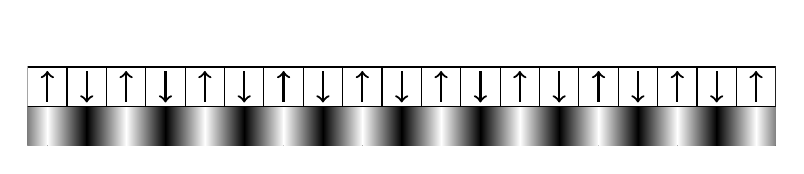
\begin{tikzpicture}
	\clip (-0.25, 0) rectangle (9.25, 1.5);
	% Settings
	\pgfmathsetmacro{\numstripes}{20}
	\pgfmathsetmacro{\stripeheight}{0.5}
	\pgfmathsetmacro{\imagewidth}{10}
	% /Settings
	\pgfmathsetmacro{\stripewidth}{\imagewidth/\numstripes}
	\foreach \idx in {0,...,\numstripes}{
		\pgfmathsetmacro{\a}{(\idx-1)*\stripewidth}
		\pgfmathsetmacro{\b}{(\idx)*\stripewidth}
		\pgfmathparse{int(mod(\idx,2))}
		\ifnum\pgfmathresult=0{\fill[left color=black, right color=white] (\a, 0) rectangle (\b, \stripeheight);}
		\else{\fill[left color=white, right color=black] (\a, 0) rectangle (\b, \stripeheight);}\fi
	}
	\begin{scope}[scale=0.5]
	\pgfmathsetmacro{\angle}{180}
	\pgfmathsetmacro{\startangle}{90}
	\foreach \idx in {0,1,...,19} {
		\pgfmathsetmacro{\anglevalue}{\startangle+\idx*\angle}
		\pgfmathsetmacro{\x}{\idx+0.4*cos(\anglevalue)}
		\pgfmathsetmacro{\a}{\idx-0.4*cos(\anglevalue)}
		\pgfmathsetmacro{\y}{1.5+0.4*sin(\anglevalue)}
		\pgfmathsetmacro{\b}{1.5+-0.4*sin(\anglevalue)}
		\draw[thick,<-] (\x, \y) -- (\a, \b);
	}
	\foreach \idx in {0,1,...,19} {
		\draw ($(\idx,0)+(-0.5,1)$) rectangle ($(\idx,0)+(0.5,2)$);
	}
	\end{scope}
\end{tikzpicture}
		\endgroup
	\end{center}
	
	\begin{itemize}
		\item Lower phase shift $\sim$ slower gray value transition
		\item Higher phase shift $\sim$ faster gray value transition
	\end{itemize}
\end{frame}

\begin{frame}
	\frametitle{And now the dreaded math part\ldots}
	
	\begin{itemize}
		\item Phase pattern: function that maps offset in left-right direction $x$ to a complex number of magnitude 1 and an angle dependent on $x$ and the phase shift $k$ corresponding to the gradient field strength
		$$p_k(x) = \mathsf e^{\mathsf ikx} = \cos(kx) + \mathsf i \sin(kx)$$
		
		\item<2> Measure similarity between pattern $p_k(x)$ and image $f(x)$: pointwise multiplication and summation
		\item<2> Result is the measured net magnetization $m(k)$ for phase shift $k$:
		\begin{align*}
			m(k) &= \int f(x)p_k(x)\ \mathsf dx \\
			     &= \int f(x)\mathsf e^{\mathsf ikx}\ \mathsf dx
		\end{align*}
	\end{itemize}
\end{frame}

\begin{frame}
	\frametitle{And now the dreaded math part\ldots}
	\begin{itemize}
		\item Result is the measured net magnetization $m(k)$ for phase shift $k$:
		\begin{align*}
			m(k) &= \int f(x)p_k(x)\ \mathsf dx \\
			     &= \int f(x)\mathsf e^{\mathsf ikx}\ \mathsf dx
		\end{align*}
		
		\item Now wait a second! We've seen that before!
		\item<2> $f(x)$ is just the Fourier transform of $m(k)$
		\item<2> Spatial encoding performs a Fourier decomposition of the image
	\end{itemize}
\end{frame}

\begin{frame}
	\frametitle{Generalization to $n$-D}
	
	\begin{itemize}
		\item Apply gradient fields in multiple directions to generate multi-dimensional phase patterns
		\item 2-D example: left-right and anterior-posterior encoding
	\end{itemize}
	\begin{center}
		\begingroup
		\tikzset{every picture/.style={scale=0.7}}
		\tikzsetnextfilename{mr_spatial_encoding_2d}
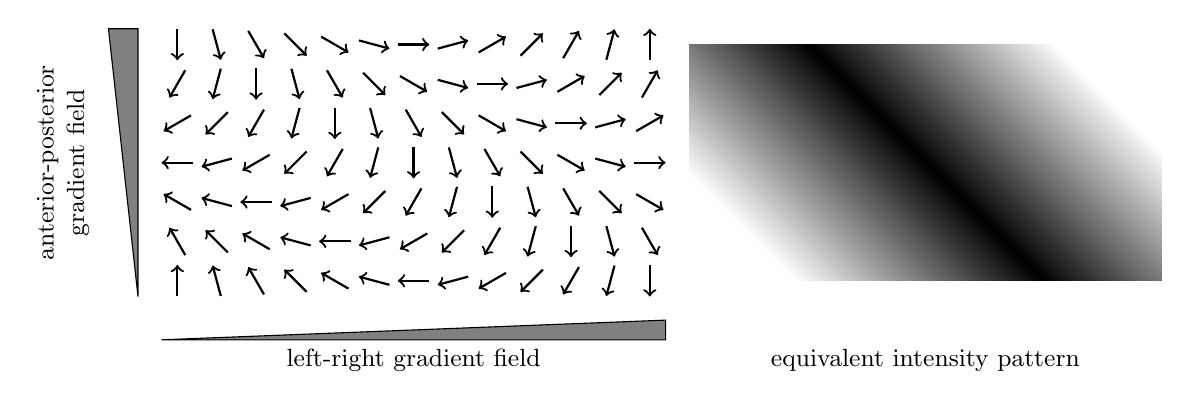
\begin{tikzpicture}[scale=0.5]
	\pgfmathsetmacro{\anglex}{15}
	\pgfmathsetmacro{\angley}{30}
	\pgfmathsetmacro{\startangle}{90}
	\foreach \idx in {0,1,...,12} {
		\foreach \idy in {0,1,...,6} {
			\pgfmathsetmacro{\anglevalue}{\startangle+\idx*\anglex+\idy*\angley}
			\pgfmathsetmacro{\x}{\idx+0.4*cos(\anglevalue)}
			\pgfmathsetmacro{\a}{\idx-0.4*cos(\anglevalue)}
			\pgfmathsetmacro{\y}{\idy+0.4*sin(\anglevalue)}
			\pgfmathsetmacro{\b}{\idy-0.4*sin(\anglevalue)}
			\draw[thick,<-] (\x, \y) -- (\a, \b);
		}
	}
	\begin{scope}[xshift=13cm]
		%\clip (-0.25, 0) rectangle (19.25, 2);
		\fill[left color=white, right color=white, middle color=black, shading angle=135] (0, 0) rectangle (12, 6);
		\coordinate (B) at (6, 3);
	\end{scope}
	\draw[fill=gray] (-0.4, -1.5) -- node (A) [below, font=\small] {left-right gradient field} (12.4, -1.5) -- (12.4, -1.0) -- cycle;
	\draw[fill=gray] (-1, -0.4) -- node [sloped, above=0.5cm, font=\small] {\parbox{3cm}{\centering anterior-posterior \\ gradient field}} (-1, 6.4) -- (-1.75, 6.4) -- cycle;
	\draw (A -| B) node [font=\small] {equivalent intensity pattern};
\end{tikzpicture}
		\endgroup
	\end{center}
\end{frame}

\begin{frame}
	\frametitle{Generalization to $n$-D}
	
	\begin{itemize}
		\item Spatial location is now a vector $\vec x \in \mathbb R^n$
		\item Combine phase shifts in each dimension into a vector $\vec k \in \mathbb R^n$
		\item Phase pattern now uses the scalar product of these vectors:
		$$p_{\vec k}(\vec x) = \mathsf e^{\mathsf i \langle \vec x, \vec k \rangle} = \cos\left( \sum_{j=1}^n x_j k_j \right) + \mathsf i \sin \left( \sum_{j=1}^n x_j k_j \right)$$
		\item Reconstruction with the $n$-D Fourier transform:
		\begin{align*}
			m(\vec k) &= \int f(\vec x) p_{\vec k}(\vec x)\ \mathsf d\vec x \\
			          &= \int f(\vec x) e^{\mathsf i \langle \vec x, \vec k \rangle}\ \mathsf d\vec x
		\end{align*}
	\end{itemize}
\end{frame}

% subsection spatial_encoding (end)



\subsection{$\vec k$-space} % (fold)
\label{sub:k_space}

\begin{frame}
	\frametitle{$\vec k$-Space}
	
	\begin{itemize}
		\item In the MR community: Fourier space $\sim$ $\vec k$-space
		\item Purpose of an MRI examination: fill the $\vec k$-space with data so image reconstruction can be performed
		\item We've already seen a 1-D $k$-space:
	\end{itemize}
	
	\begin{center}
		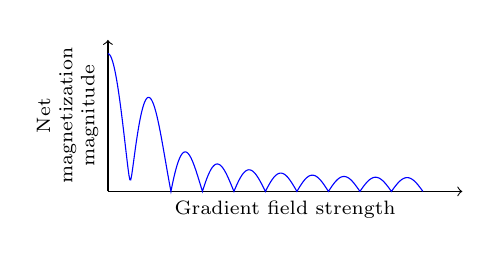
\begin{tikzpicture}[yscale=3.5]
   		\draw[->] (0, 0) -- node [below, font=\scriptsize] {\parbox{3cm}{\centering Gradient field strength}} (4.5, 0);
   		\draw[->] (0, 0) -- node [above, sloped, font=\scriptsize] {\parbox{2cm}{\centering Net magnetization \\ magnitude}} (0, 0.55);
   		\draw[blue] (0.000000, 0.500000)
    -- (0.011111, 0.498993)
    -- (0.022222, 0.495976)
    -- (0.033333, 0.490965)
    -- (0.044444, 0.483986)
    -- (0.055556, 0.475075)
    -- (0.066667, 0.464278)
    -- (0.077778, 0.451650)
    -- (0.088889, 0.437256)
    -- (0.100000, 0.421170)
    -- (0.111111, 0.403476)
    -- (0.122222, 0.384266)
    -- (0.133333, 0.363639)
    -- (0.144444, 0.341703)
    -- (0.155556, 0.318575)
    -- (0.166667, 0.294377)
    -- (0.177778, 0.269242)
    -- (0.188889, 0.243312)
    -- (0.200000, 0.216740)
    -- (0.211111, 0.189698)
    -- (0.222222, 0.162386)
    -- (0.233333, 0.135060)
    -- (0.244444, 0.108093)
    -- (0.255556, 0.082163)
    -- (0.266667, 0.058836)
    -- (0.277778, 0.042508)
    -- (0.288889, 0.041785)
    -- (0.300000, 0.056652)
    -- (0.311111, 0.078109)
    -- (0.322222, 0.101488)
    -- (0.333333, 0.125154)
    -- (0.344444, 0.148430)
    -- (0.355556, 0.170963)
    -- (0.366667, 0.192530)
    -- (0.377778, 0.212971)
    -- (0.388889, 0.232162)
    -- (0.400000, 0.250000)
    -- (0.411111, 0.266400)
    -- (0.422222, 0.281290)
    -- (0.433333, 0.294611)
    -- (0.444444, 0.306315)
    -- (0.455556, 0.316366)
    -- (0.466667, 0.324735)
    -- (0.477778, 0.331407)
    -- (0.488889, 0.336374)
    -- (0.500000, 0.339639)
    -- (0.511111, 0.341215)
    -- (0.522222, 0.341122)
    -- (0.533333, 0.339392)
    -- (0.544444, 0.336064)
    -- (0.555556, 0.331184)
    -- (0.566667, 0.324809)
    -- (0.577778, 0.317001)
    -- (0.588889, 0.307829)
    -- (0.600000, 0.297371)
    -- (0.611111, 0.285709)
    -- (0.622222, 0.272931)
    -- (0.633333, 0.259128)
    -- (0.644444, 0.244400)
    -- (0.655556, 0.228845)
    -- (0.666667, 0.212568)
    -- (0.677778, 0.195676)
    -- (0.688889, 0.178275)
    -- (0.700000, 0.160475)
    -- (0.711111, 0.142386)
    -- (0.722222, 0.124116)
    -- (0.733333, 0.105773)
    -- (0.744444, 0.087465)
    -- (0.755556, 0.069296)
    -- (0.766667, 0.051369)
    -- (0.777778, 0.033781)
    -- (0.788889, 0.016628)
    -- (0.800000, 0.000000)
    -- (0.811111, 0.016017)
    -- (0.822222, 0.031342)
    -- (0.833333, 0.045901)
    -- (0.844444, 0.059624)
    -- (0.855556, 0.072450)
    -- (0.866667, 0.084323)
    -- (0.877778, 0.095194)
    -- (0.888889, 0.105021)
    -- (0.900000, 0.113769)
    -- (0.911111, 0.121412)
    -- (0.922222, 0.127930)
    -- (0.933333, 0.133309)
    -- (0.944444, 0.137547)
    -- (0.955556, 0.140643)
    -- (0.966667, 0.142609)
    -- (0.977778, 0.143461)
    -- (0.988889, 0.143221)
    -- (1.000000, 0.141919)
    -- (1.011111, 0.139592)
    -- (1.022222, 0.136282)
    -- (1.033333, 0.132034)
    -- (1.044444, 0.126904)
    -- (1.055556, 0.120946)
    -- (1.066667, 0.114224)
    -- (1.077778, 0.106802)
    -- (1.088889, 0.098750)
    -- (1.100000, 0.090137)
    -- (1.111111, 0.081040)
    -- (1.122222, 0.071533)
    -- (1.133333, 0.061693)
    -- (1.144444, 0.051597)
    -- (1.155556, 0.041325)
    -- (1.166667, 0.030953)
    -- (1.177778, 0.020558)
    -- (1.188889, 0.010216)
    -- (1.200000, 0.000000)
    -- (1.211111, 0.010018)
    -- (1.222222, 0.019769)
    -- (1.233333, 0.029187)
    -- (1.244444, 0.038211)
    -- (1.255556, 0.046782)
    -- (1.266667, 0.054846)
    -- (1.277778, 0.062353)
    -- (1.288889, 0.069259)
    -- (1.300000, 0.075523)
    -- (1.311111, 0.081112)
    -- (1.322222, 0.085995)
    -- (1.333333, 0.090149)
    -- (1.344444, 0.093557)
    -- (1.355556, 0.096204)
    -- (1.366667, 0.098085)
    -- (1.377778, 0.099198)
    -- (1.388889, 0.099547)
    -- (1.400000, 0.099141)
    -- (1.411111, 0.097996)
    -- (1.422222, 0.096131)
    -- (1.433333, 0.093571)
    -- (1.444444, 0.090345)
    -- (1.455556, 0.086487)
    -- (1.466667, 0.082035)
    -- (1.477778, 0.077030)
    -- (1.488889, 0.071517)
    -- (1.500000, 0.065544)
    -- (1.511111, 0.059162)
    -- (1.522222, 0.052424)
    -- (1.533333, 0.045384)
    -- (1.544444, 0.038098)
    -- (1.555556, 0.030624)
    -- (1.566667, 0.023019)
    -- (1.577778, 0.015342)
    -- (1.588889, 0.007650)
    -- (1.600000, 0.000000)
    -- (1.611111, 0.007551)
    -- (1.622222, 0.014949)
    -- (1.633333, 0.022141)
    -- (1.644444, 0.029077)
    -- (1.655556, 0.035707)
    -- (1.666667, 0.041987)
    -- (1.677778, 0.047874)
    -- (1.688889, 0.053329)
    -- (1.700000, 0.058317)
    -- (1.711111, 0.062806)
    -- (1.722222, 0.066770)
    -- (1.733333, 0.070184)
    -- (1.744444, 0.073029)
    -- (1.755556, 0.075291)
    -- (1.766667, 0.076959)
    -- (1.777778, 0.078029)
    -- (1.788889, 0.078497)
    -- (1.800000, 0.078368)
    -- (1.811111, 0.077649)
    -- (1.822222, 0.076352)
    -- (1.833333, 0.074492)
    -- (1.844444, 0.072089)
    -- (1.855556, 0.069167)
    -- (1.866667, 0.065752)
    -- (1.877778, 0.061877)
    -- (1.888889, 0.057573)
    -- (1.900000, 0.052878)
    -- (1.911111, 0.047830)
    -- (1.922222, 0.042470)
    -- (1.933333, 0.036842)
    -- (1.944444, 0.030990)
    -- (1.955556, 0.024960)
    -- (1.966667, 0.018799)
    -- (1.977778, 0.012554)
    -- (1.988889, 0.006271)
    -- (2.000000, 0.000000)
    -- (2.011111, 0.006214)
    -- (2.022222, 0.012325)
    -- (2.033333, 0.018288)
    -- (2.044444, 0.024060)
    -- (2.055556, 0.029599)
    -- (2.066667, 0.034866)
    -- (2.077778, 0.039824)
    -- (2.088889, 0.044438)
    -- (2.100000, 0.048678)
    -- (2.111111, 0.052513)
    -- (2.122222, 0.055920)
    -- (2.133333, 0.058876)
    -- (2.144444, 0.061363)
    -- (2.155556, 0.063366)
    -- (2.166667, 0.064873)
    -- (2.177778, 0.065878)
    -- (2.188889, 0.066378)
    -- (2.200000, 0.066371)
    -- (2.211111, 0.065863)
    -- (2.222222, 0.064860)
    -- (2.233333, 0.063375)
    -- (2.244444, 0.061422)
    -- (2.255556, 0.059019)
    -- (2.266667, 0.056187)
    -- (2.277778, 0.052952)
    -- (2.288889, 0.049339)
    -- (2.300000, 0.045379)
    -- (2.311111, 0.041105)
    -- (2.322222, 0.036549)
    -- (2.333333, 0.031750)
    -- (2.344444, 0.026743)
    -- (2.355556, 0.021568)
    -- (2.366667, 0.016266)
    -- (2.377778, 0.010877)
    -- (2.388889, 0.005441)
    -- (2.400000, 0.000000)
    -- (2.411111, 0.005405)
    -- (2.422222, 0.010734)
    -- (2.433333, 0.015948)
    -- (2.444444, 0.021007)
    -- (2.455556, 0.025876)
    -- (2.466667, 0.030518)
    -- (2.477778, 0.034901)
    -- (2.488889, 0.038992)
    -- (2.500000, 0.042764)
    -- (2.511111, 0.046189)
    -- (2.522222, 0.049244)
    -- (2.533333, 0.051909)
    -- (2.544444, 0.054165)
    -- (2.555556, 0.055997)
    -- (2.566667, 0.057396)
    -- (2.577778, 0.058352)
    -- (2.588889, 0.058861)
    -- (2.600000, 0.058922)
    -- (2.611111, 0.058536)
    -- (2.622222, 0.057710)
    -- (2.633333, 0.056451)
    -- (2.644444, 0.054771)
    -- (2.655556, 0.052685)
    -- (2.666667, 0.050212)
    -- (2.677778, 0.047371)
    -- (2.688889, 0.044187)
    -- (2.700000, 0.040684)
    -- (2.711111, 0.036890)
    -- (2.722222, 0.032836)
    -- (2.733333, 0.028554)
    -- (2.744444, 0.024076)
    -- (2.755556, 0.019438)
    -- (2.766667, 0.014674)
    -- (2.777778, 0.009822)
    -- (2.788889, 0.004918)
    -- (2.800000, 0.000000)
    -- (2.811111, 0.004896)
    -- (2.822222, 0.009732)
    -- (2.833333, 0.014474)
    -- (2.844444, 0.019084)
    -- (2.855556, 0.023530)
    -- (2.866667, 0.027778)
    -- (2.877778, 0.031798)
    -- (2.888889, 0.035560)
    -- (2.900000, 0.039036)
    -- (2.911111, 0.042203)
    -- (2.922222, 0.045037)
    -- (2.933333, 0.047518)
    -- (2.944444, 0.049630)
    -- (2.955556, 0.051357)
    -- (2.966667, 0.052688)
    -- (2.977778, 0.053615)
    -- (2.988889, 0.054132)
    -- (3.000000, 0.054237)
    -- (3.011111, 0.053931)
    -- (3.022222, 0.053217)
    -- (3.033333, 0.052103)
    -- (3.044444, 0.050598)
    -- (3.055556, 0.048714)
    -- (3.066667, 0.046469)
    -- (3.077778, 0.043878)
    -- (3.088889, 0.040964)
    -- (3.100000, 0.037750)
    -- (3.111111, 0.034259)
    -- (3.122222, 0.030521)
    -- (3.133333, 0.026563)
    -- (3.144444, 0.022417)
    -- (3.155556, 0.018114)
    -- (3.166667, 0.013686)
    -- (3.177778, 0.009169)
    -- (3.188889, 0.004595)
    -- (3.200000, 0.000000)
    -- (3.211111, 0.004582)
    -- (3.222222, 0.009115)
    -- (3.233333, 0.013567)
    -- (3.244444, 0.017904)
    -- (3.255556, 0.022092)
    -- (3.266667, 0.026103)
    -- (3.277778, 0.029904)
    -- (3.288889, 0.033469)
    -- (3.300000, 0.036771)
    -- (3.311111, 0.039786)
    -- (3.322222, 0.042492)
    -- (3.333333, 0.044869)
    -- (3.344444, 0.046901)
    -- (3.355556, 0.048571)
    -- (3.366667, 0.049870)
    -- (3.377778, 0.050788)
    -- (3.388889, 0.051318)
    -- (3.400000, 0.051458)
    -- (3.411111, 0.051208)
    -- (3.422222, 0.050570)
    -- (3.433333, 0.049549)
    -- (3.444444, 0.048155)
    -- (3.455556, 0.046399)
    -- (3.466667, 0.044294)
    -- (3.477778, 0.041857)
    -- (3.488889, 0.039107)
    -- (3.500000, 0.036066)
    -- (3.511111, 0.032757)
    -- (3.522222, 0.029204)
    -- (3.533333, 0.025437)
    -- (3.544444, 0.021482)
    -- (3.555556, 0.017372)
    -- (3.566667, 0.013136)
    -- (3.577778, 0.008806)
    -- (3.588889, 0.004417)
    -- (3.600000, 0.000000)
    -- (3.611111, 0.004410)
    -- (3.622222, 0.008781)
    -- (3.633333, 0.013080)
    -- (3.644444, 0.017273)
    -- (3.655556, 0.021331)
    -- (3.666667, 0.025221)
    -- (3.677778, 0.028916)
    -- (3.688889, 0.032387)
    -- (3.700000, 0.035608)
    -- (3.711111, 0.038556)
    -- (3.722222, 0.041209)
    -- (3.733333, 0.043546)
    -- (3.744444, 0.045550)
    -- (3.755556, 0.047207)
    -- (3.766667, 0.048505)
    -- (3.777778, 0.049433)
    -- (3.788889, 0.049986)
    -- (3.800000, 0.050159)
    -- (3.811111, 0.049951)
    -- (3.822222, 0.049364)
    -- (3.833333, 0.048403)
    -- (3.844444, 0.047075)
    -- (3.855556, 0.045390)
    -- (3.866667, 0.043362)
    -- (3.877778, 0.041006)
    -- (3.888889, 0.038340)
    -- (3.900000, 0.035383)
    -- (3.911111, 0.032159)
    -- (3.922222, 0.028693)
    -- (3.933333, 0.025009)
    -- (3.944444, 0.021136)
    -- (3.955556, 0.017104)
    -- (3.966667, 0.012942)
    -- (3.977778, 0.008683)
    -- (3.988889, 0.004358)
    -- (4.000000, 0.000000);
\end{tikzpicture}
	\end{center}
	
\end{frame}

\begin{frame}
	\frametitle{2-D $\vec k$-Space}
	
	\begin{itemize}
		\item 2-D $\vec k$-space with phase patterns associated with some positions:
	\end{itemize}
	
	\vspace{-2ex}
	
	\begin{center}
		\newlength\imagewidth
\newlength\imagescale
\pgfmathsetlength{\imagewidth}{0.3\linewidth}
\pgfmathsetlength{\imagescale}{\imagewidth/128}
\tikzsetnextfilename{mr_k_space}
\begin{tikzpicture}[x=\imagescale,y=-\imagescale]
	\node[anchor=north west,inner sep=0pt,outer sep=0pt] (ksp) at (-0.5,-0.5)
   {\includegraphics[width=\imagewidth]{images/kspace}};
	\draw[thick,->] (-4, 64) -- (131, 64) node [right] {$k_x$};
	\draw[thick,->] (64, 131) -- (64, -4) node [above] {$k_y$};
	\filldraw (64, 54) coordinate (ksp1) circle (1.5pt);
	\filldraw (69, 64) coordinate (ksp2) circle (1.5pt);
	\filldraw (60, 56) coordinate (ksp3) circle (1.5pt);
	\filldraw (54, 79) coordinate (ksp4) circle (1.5pt);
	
	\node[anchor=north west,inner sep=0pt,outer sep=0pt] (kspf1) at ($(ksp.north east) + (1cm, 0)$) {\includegraphics[width=.1509\linewidth]{images/spatialfreq_0_10}};
	\draw[->, shorten >=1mm] (ksp1) -- (kspf1.west);
	\node[anchor=south west,inner sep=0pt,outer sep=0pt] (kspf2) at ($(ksp.south east) + (1cm, 0)$) {\includegraphics[width=.1509\linewidth]{images/spatialfreq_5_0}};
	\draw[->, shorten >=1mm] (ksp2) -- (kspf2.west);
	\node[anchor=north east,inner sep=0pt,outer sep=0pt] (kspf3) at ($(ksp.north west) - (1cm, 0)$) {\reflectbox{\includegraphics[width=.1509\linewidth]{images/spatialfreq_-4_8}}};
	\draw[->, shorten >=1mm] (ksp3) -- (kspf3.east);
	\node[anchor=south east,inner sep=0pt,outer sep=0pt] (kspf4) at ($(ksp.south west) - (1cm, 0)$) {\reflectbox{\includegraphics[width=.1509\linewidth]{images/spatialfreq_-10_-15}}};
	\draw[->, shorten >=1mm] (ksp4) -- (kspf4.east);
\end{tikzpicture}

	\end{center}
\end{frame}

% subsection k_space (end)



\subsection{Slice-selective vs.~Volume-selective 3-D Imaging} % (fold)
\label{sub:slice_selective_vs_volume_selective_3_d_imaging}

\begin{frame}
	\frametitle{3-D Imaging}
	
	Two options for 3-D imaging:
	
	\vspace{-2ex}
	
	\begin{columns}[t,onlytextwidth]

	    \column{0.47\textwidth}
	    \begin{block}{Slice Selective}
	        \begin{itemize}
	            \small
	            \item Use slice selection to acquire stack of 2-D slices
				\item Localization within each slice using 2-D spatial encoding
				\item Characteristics:
				\begin{itemize}
					\item Commonly anisotropic resolution
					\item High in-plane resolution
					\item Low through-plane resolution (thick slices)
				\end{itemize}
	        \end{itemize}
	    \end{block}

	    \column{0.5\textwidth}
		\uncover<2>{
	    \begin{block}{Volume Selective}
	        \begin{itemize}
	            \small
	            \item Excite the entire volume without slice selection
				\item Perform 3-D spatial encoding for localization
				\item Characteristics:
				\begin{itemize}
					\item Commonly isotropic resolution, not as high as slice-selective in-plane
					\item Inherent SNR benefit: more \hydrogen{} nuclei resonate
				\end{itemize}
	        \end{itemize}
	    \end{block}}

	\end{columns}
\end{frame}

% subsection slice_selective_vs_volume_selective_3_d_imaging (end)

% section principles_of_magnetic_resonance_imaging (end)



\section{Advanced Applications} % (fold)
\label{sec:advanced_applications}

\begin{frame}
	\frametitle{Advanced Applications}
	
	\begin{itemize}
		\item Going beyond simple morphological \longtime{}/\transtime{}/PD imaging
		\item Spectrally selective excitation
		\begin{itemize}
			\item \transtime{} preparation for better coronary artery depiction
			\item Water-fat separation
		\end{itemize}
		\item Functional imaging
		\begin{itemize}
			\item Non-contrast angiography
			\item BOLD imaging
		\end{itemize}
	\end{itemize}
\end{frame}



\subsection{Spectrally Selective Excitation} % (fold)
\label{sub:spectrally_selective_excitation}

\begin{frame}
	\frametitle{\transtime{} Preparation for Coronary Angiography}
	
	\begin{itemize}
		\item Improve contrast between arterial blood and myocardium
		\item Relies on difference in \transtime{} constants
		\item Decrease magnetizability of myocardial tissue and venous blood
		\item Arterial blood remains mostly unaffected
	\end{itemize}
	
	\begin{center}
		\tikzsetnextfilename{mr_t2_preparation_constants}
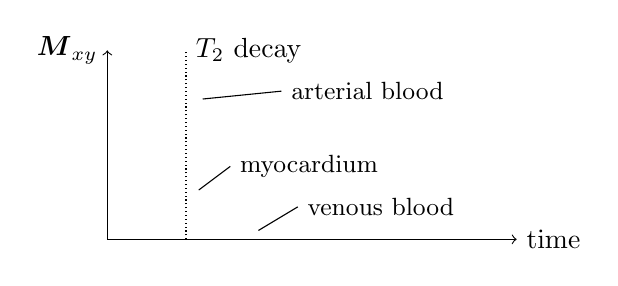
\begin{tikzpicture}[yscale=2]
	\draw[->] (0, 0) -- (0, 1.2) node [left] {\magntrans{}};
	\draw[->] (0, 0) -- (5.2, 0) node [right] {time};
	\draw[densely dotted] (1, 0) -- (1, 1.2) node [right] {\transtime{} decay};
	\draw[domain=0:5,samples=100,very thick] plot[id=mr_t2_arterial] function{exp(-x/10.5)};
	\draw[domain=0:5,samples=100,very thick,densely dotted] plot[id=mr_t2_venous] function{exp(-x*1.5)};
	\draw[domain=0:5,samples=100,very thick,densely dashed] plot[id=mr_t2_myocardium] function{exp(-x)};
	\draw (1.16162, 0.31298) -- +(0.4, 0.15) node [right, font=\small] {myocardium};
	\draw (1.21212, 0.89097) -- +(1, 0.05) node [right, font=\small] {arterial blood};
	\draw (1.91919, 0.05620) -- +(0.5, 0.15) node [right, font=\small] {venous blood};
\end{tikzpicture}
	\end{center}
\end{frame}

\begin{frame}
	\frametitle{\transtime{} Preparation for Coronary Angiography}
	
	\begin{columns}[onlytextwidth,c]
		\column{.5\linewidth}
		\begin{center}
			\includegraphics[width=.65\linewidth]{images/without_t2prep}
			
			Without \transtime{} preparation
		\end{center}
		
		\column{.5\linewidth}
		\begin{center}
			\includegraphics[width=.65\linewidth]{images/with_t2prep}
			
			With \transtime{} preparation
		\end{center}
	\end{columns}
	
	\vspace{1ex}
	
	{\scriptsize Image source: Reza Nezafat et al. \emph{B1-Insensitive T2 Preparation for Improved Coronary Magnetic Resonance Angiography at $3\,\textsf{T}$}. Magn Reson Med 55:858–864 (2006).}
\end{frame}

\begin{frame}
	\frametitle{Hydrogens in Water and Fat}
	\framesubtitle{Differences between hydrogens bound in water and fat}

\begin{figure}%
\includegraphics[height=4cm]{images/hydrogen_in_water_fat.png}%
\end{figure}
%
\begin{itemize}
		\item Molecule structures of water and fat (triglycerides) are different
			\begin{itemize}
			\item Fat: large molecules, high shielding $\rightarrow$ short T1
			\item Water: small molecules, less shielding $\rightarrow$ long T1
			\item Resonance frequency differs $\rightarrow$ chemical shift artifacts
			\end{itemize}
	\end{itemize}
\end{frame}

\begin{frame}
\frametitle{Fat-Suppression}
%\framesubtitle{Fat suppression}

\begin{itemize}
		\item Fat is hyperintense in many contrasts
			\begin{itemize}
		\item Obscures pathologies by decreasing contrast of non-fatty tissue
		\item Increases motion artifacts
		\item $\rightarrow$ Fat suppression, water excitation or water-fat separation
		\end{itemize}
\end{itemize}

	\begin{figure}
		\centering
		\subcaptionbox*{Liver: no suppression}{\includegraphics[height=3.6cm]{images/NoFatsat.png}}
		\subcaptionbox*{Liver: fat suppression}{\includegraphics[height=3.6cm]{images/WithFatsat.png}}
				\vspace{-2.5ex}
		\caption*{\scriptsize Image source: Magnets, Flows and Artifacts, Siemens 2004}
	\end{figure}

\end{frame}

\begin{frame}
%\frametitle{Water-Fat Imaging}
\frametitle{Water-Fat Separation}
\begin{itemize}
	\item Separation via chemical shift encoding: pure water and fat signal
	\begin{itemize}
		\item Water signal without residual fat $\rightarrow$ lesion detection
		\item Fat quantification $\rightarrow$ diagnosis of fat-related pathologies
	\end{itemize}
	%\item Cleanly separated water and fat images $\rightarrow$ diagnostically useful
\end{itemize}

	\begin{figure}
		\centering
		\subcaptionbox*{Water signal}{\includegraphics[height=3.7cm]{images/water.png}}
		\subcaptionbox*{Fat signal}{\includegraphics[height=3.7cm]{images/fat.png}}
	\end{figure}
	\vspace{-0.5ex}

\end{frame}

\begin{frame}
\frametitle{Fat Quantification}
%\framesubtitle{Fat fraction }
\begin{itemize}
	\item Relative water-fat composition as quantitative biomarker
		\begin{itemize}
			\item Diagnosis of liver fibrosis, hepatic steatosis, HIV, ...
			\item Fat fraction = Fat/(Water+Fat) e.g. pathological liver > 6 \%
		\end{itemize}
\end{itemize}
\vspace{-0.1ex}

	\begin{figure}
		\centering
		\subcaptionbox*{}{\includegraphics[height=4cm]{images/fat_quantification.png}}
\end{figure}
\vspace{-4ex}

\centering
\fontsize{8.4}{8.4}\selectfont
Liver fat assessment before and after drug treatment \\ Image source: Reeder et al., MRM 34.4 (2011): 729-749
\end{frame}

% subsection spectrally_selective_excitation (end)



\subsection{Functional Imaging} % (fold)
\label{sub:functional_imaging}

\begin{frame}
	\frametitle{Non-Contrast Angiography}
	
	\begin{itemize}
		\item MR angiography typically relies on Gadolinium as contrast agent
		\item Time-of-Flight angiography
		\begin{itemize}
			\item Saturate magnetization within a slice
			\item Inflow: blood vessels carry non-saturated blood into imaging plane
			\item Subsequent imaging shows highly contrasted blood vessels
		\end{itemize}
	\end{itemize}
	
	\begin{columns}[onlytextwidth,c]
		\column{.5\linewidth}
		\begin{center}
			\begingroup
			\tikzset{every picture/.style={scale=0.6}}
			\input{tikz/tof_angiography_saturation.tikz}
			\endgroup
		\end{center}
		
		\column{.5\linewidth}
		\begin{center}
			\begingroup
			\tikzset{every picture/.style={scale=0.6,font=\scriptsize}}
			\tikzsetnextfilename{mr_tof_angiography_inflow}
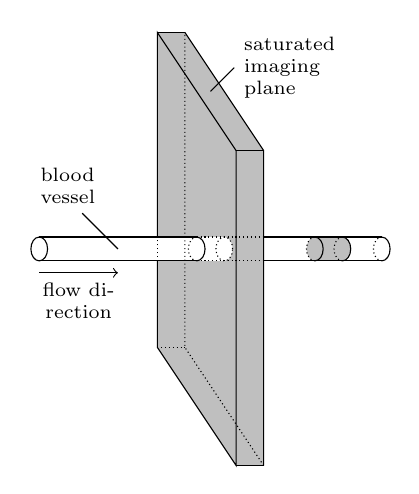
\begin{tikzpicture}
	\fill[lightgray] (3.5, -1ex) -- (3.85, -1ex) arc (-90:90:0.7ex and 1ex) -- (3.5, 1ex) arc (90:270:0.7ex and 1ex);
	
	\draw (2.85, 1ex) -- (4.35, 1ex);
	\draw (2.85, -1ex) -- (4.35, -1ex);
	\node (c) at (4.35, 0) {};
	\begin{scope}[shift={(c)}]
		\draw (0, -1ex) arc (-90:90:0.7ex and 1ex);
		\draw[densely dotted] (0, 1ex) arc (90:270:0.7ex and 1ex);
	\end{scope}
	\node (d) at (3.5, 0) {};
	\begin{scope}[shift={(d)}]
		\draw (0, -1ex) arc (-90:90:0.7ex and 1ex);
		\draw[densely dotted] (0, 1ex) arc (90:270:0.7ex and 1ex);
	\end{scope}
	\node (e) at (3.85, 0) {};
	\begin{scope}[shift={(e)}]
		\draw (0, -1ex) arc (-90:90:0.7ex and 1ex);
		\draw[densely dotted] (0, 1ex) arc (90:270:0.7ex and 1ex);
	\end{scope}

	\fill[lightgray] (1.5,  2.75) -- (1.85,  2.75) -- (2.85, 1.25) -- (2.85, -2.75) -- (2.5, -2.75) -- (1.5, -1.25) -- cycle;

	\fill[white] (0, -1ex) -- (2.35, -1ex) arc (-90:90:0.7ex and 1ex) -- (0, 1ex) arc (90:270:0.7ex and 1ex);

	\draw (0, 0) ellipse (0.7ex and 1ex);
	\node (a) at (2, 0) {};
	\begin{scope}[shift={(a)}]
		\draw (0, -1ex) arc (-90:90:0.7ex and 1ex);
		\draw[densely dotted] (0, 1ex) arc (90:270:0.7ex and 1ex);
	\end{scope}
	\draw[densely dotted] (2.35, 0) ellipse (0.7ex and 1ex);

	\draw (0, 1ex) -- (2, 1ex);
	\draw[densely dotted] (2, 1ex) -- (2.85, 1ex);

	\draw (0, -1ex) -- (2, -1ex);
	\draw[densely dotted] (2, -1ex) -- (2.85, -1ex);

	\draw (2.5, 1.25) -- (2.5, -2.75) -- (1.5, -1.25) -- (1.5, -1ex);
	\draw[densely dotted] (1.5, -1ex) -- (1.5, 1ex);
	\draw (1.5, 1ex) -- (1.5, 2.75) -- (2.5, 1.25);
	\draw (1.85, 2.75) -- (2.85, 1.25) -- (2.85, -2.75);
	\draw[densely dotted] (2.85, -2.75) -- (1.85, -1.25) -- (1.85, 2.75);
	\draw (2.5,  1.25) -- (2.85,  1.25);
	\draw (2.5, -2.75) -- (2.85, -2.75);
	\draw (1.5,  2.75) -- (1.85,  2.75);
	\draw[densely dotted] (1.5, -1.25) -- (1.85, -1.25);
	\draw (2.175, 2) -- ++ (2ex, 2ex) node [right, font=\scriptsize] {\parbox{10ex}{saturated imaging plane}};
	\draw (1, 0) -- ++ (-3ex, 3ex) node [above, font=\scriptsize] {\parbox{10ex}{blood \\ vessel}};
	\draw[->] (0, -2ex) -- node [below, font=\scriptsize] {\parbox{10ex}{\centering flow direction}} (1, -2ex);
\end{tikzpicture}
			\endgroup
		\end{center}
	\end{columns}
\end{frame}

\begin{frame}
	\frametitle{Non-Contrast Angiography}
	
	\begin{center}
		\includegraphics[height=0.8\textheight]{images/mra_head}
	\end{center}
	
	\flushright
	\tiny Image source: \url{http://www.imp.uni-erlangen.de/mri/de/projects_mra.html}
\end{frame}

\begin{frame}
	\frametitle{The BOLD Effect and fMRI}

		\begin{itemize}
		\item Functional MRI often aims to visualize neuronal brain activity
		\item Idea: increased neuronal activity $\rightarrow$ local oxygen depletion $\rightarrow$ overcompensation $\rightarrow$ high concentration of oxygenated blood
		\item The blood-oxygenation-level dependent (BOLD) effect correlates oxygenated blood with a high \inhomogtime{} constant
		\item By comparing images during stimulus and resting state on many repetitions, active regions for that stimulus can be identified
		\end{itemize}
		
				\begin{figure}
	\includegraphics[height=2.6cm]{images/fmri_bold.jpg}
	\end{figure}
	\vspace{-1ex}
	\centering
\fontsize{7.5}{8.4}\selectfont
Image source: \url{http://www.fmrib.ox.ac.uk}
	%{\scriptsize(Image source: \url{http://www.fmrib.ox.ac.uk})}
	
\end{frame}

\begin{frame}
	\frametitle{fMRI Study: Gender Differences}
	%\framesubtitle{Task: Are two presented 3D drawings from the same shape?}
	
			\begin{itemize}
		\item Stimulus for subjects: decide whether two presented 3D drawings are from the same shape
		\item Study outcome: males and females activate different brain areas for solving mental rotation tasks
		\end{itemize}
	
	\begin{figure}
	\includegraphics[height=3cm]{images/fmri_men_women.png}
	\end{figure}
	
\centering
\fontsize{8}{8.4}\selectfont
Significant MR signal increases for the males after subtracting activity for the females \\during the 3-D mental rotation task\\ Source: K. Hugdahl et al., Neuropsychologia 44.9 (2006): 1575-1583
\end{frame}

% subsection functional_imaging (end)

% section advanced_applications (end)

\end{document}
